\chapter{Methods}

\section{Datasets}
In this section, we introduce some important datasets used in this thesis for model training and performance evaluation. First, we present every datasets involved in pretraining of our models. For finetuning and inference, the most interesting dataset in the context of the research of this project is the 3D+t dataset of zebrafish embryo provided by the biologists at @todo.
There are multiple challenges when working with these datasets. The most important challenge is the lack of annotated data. Even for fully annotated datasets, inter-annotator agreement is often an upper boundary for evaluation, as even for the specialist a clear annotation is sometimes not obvious. This can be due to a certain level of noise in the images or boundaries that are just inherently hard to define due to the cell type or imaging modality. This is especially the case for the non-synthetic data, provided by the Celltracking Challenge (CTC) \cite{ctc}. Next to limited annotations, 3D data can quickly blow up computational resources due to their large size. For this matter, some shifted window approach has to be considered, if the image size exceeds computational limits. Anisotropy can also can also lead to distortions in feature aquisition and performance impairments at inference, if not taken care of in each processing step. 

\subsection{Pretraining Datasets}
For pretraining our models, we want to use as many 2D cell microscopy data as we can get. The modalites range from H\&E stained histology images from various organs, over fluorescence, phase-contrast and bright-field microscopy images. Cell types range from human organ cells, to bacteria, worms, yeast and animal embryo nuclei.

\begin{itemize}
  \item BCCD: The blood cell segmentation dataset consists of blood smear images taken with a light microscope 
  (\url{https://www.kaggle.com/datasets/jeetblahiri/bccd-dataset-with-mask}). 
  There are 1,169 training and 159 validation images in the dataset, all of which were used for training.

  \item Cellpose: We used the dataset from the original Cellpose paper. It is composed from various sources. We manually selected 764 images for training.

  \item CoNIC: The CoNIC dataset consists of 4,981 H\&E images with labeled nuclei and nuclei classification 
  (\url{https://www.kaggle.com/datasets/aadimator/conic-challenge-dataset?select=data}). 
  We sorted out the images without labels and ended up with 4,841 images which we used for training.

  \item CPM15+17: CPM 15 and 17 consist of H\&E images with labeled nuclei. CPM 15 + 17 are from brain cancer patients, with 15 and 32 training images per dataset, respectively.

  \item DataScienceBowl: The 2018 DataScienceBowl dataset contains 841 images with 22 cell types and five visually similar groups. We used 670 images for training.

  \item DeepBacs: We used the following segmentation datasets from DeepBacs: S. aureus bright-field and fluorescence with 66 training patches, E. coli bright-field with 34 training images, and B. subtilis fluorescence with 90; in total 190 training images.

  \item IHC\_TMA: The IHC TMA dataset consists of TMA sections from non-small cell lung cancer patients with labeled nuclei 
  (\url{https://doi.org/10.5281/zenodo.7647846}). 
  There are 266 images, which were used for training.

  \item LiveCell: The LiveCell dataset consists of 4,704 images of 8 different cell lines collected using phase-contrast microscopy 
  (\url{https://sartorius-research.github.io/LIVECell/}). 
  We manually selected 3,699 images that have complete annotations.

  \item LynSec: LynSec consists of 699 IHC and H\&E images from lymphoma patients with labeled nuclei 
  (\url{https://zenodo.org/records/8065174}). 
  We used all images for training.

  \item NeurIPS: The NeurIPS 2022 challenge training dataset consists of 1,000 images with labeled cells from bright-field, fluorescent, phase-contrast, and differential interference contrast imaging modalities 
  (\url{https://neurips22-cellseg.grand-challenge.org/neurips22-cellseg/}). 
  We manually selected 914 images that were annotated to a satisfactory degree.

  \item NuInsSeg: The NuInsSeg dataset consists of H\&E images from 31 different human and mouse organs with labeled nuclei 
  (\url{https://www.kaggle.com/datasets/ipateam/nuinsseg}). 
  We used all 664 available images for training.

  \item Omnipose: This dataset contains a mixture of 14 bacterial species. We used 611 bacterial cell
microscopy images and discarded 118 worm images.

  \item PanNuke: The PanNuke dataset consists of 7,898 H\&E images from 19 tissue types from cancer patients with labeled nuclei and nuclei classification 
  (\url{https://warwick.ac.uk/fac/cross_fac/tia/data/pannuke}). 
  We manually selected 4,950 images that had enough annotations.

  \item TissueNet: The TissueNet dataset consists of 3 folds of 2,580, 3,118, and 1,324 images, collected using fluorescent microscopy on 6 tissue types with labeled cells and nuclei 
  (\url{https://datasets.deepcell.org/}). 
  We used all of them for training, although some appeared to have very heavy augmentations.

  \item TNBC: This dataset consists of 50 images from triple negative breast cancer patients, all of which were used for training 
  (\url{https://drive.google.com/drive/folders/1l55cv3DuY-f7-JotDN7N5nbNnjbLWchK}).

  \item YeaZ: The YeaZ dataset consists of bright-field and phase contrast images of yeast cells. We used 401 2D images from the phase contrast dataset for training, and 306 images from the bright-field dataset for training.
\end{itemize}

\subsection{Evaluation Datasets}

To test the performance of our pretrained models, we collected datasets with fully annotated stacks and others that only have partially annotated images. Unlike the pretraining data, the evaluation datasets have to be 3D. This dramatically increases annotation costs, so finding public, fully annotated datasets here is hard. Again, DDPMs could substitute this labor intense task of annotating full 3D stacks. However, since we dont rely on true 3D-training data, the few datasets available for testing are sufficient.

\subsubsection{BlastoSPIM}

BlastoSPIM contains two large-scale, high-resolution collections of annotated light-sheet images of mouse embryos.
The first dataset, \textit{BlastoSPIM 1.0}, primarily includes embryos from the 8-nuclei stage to the 64-nuclei stage, while the second dataset, \textit{BlastoSPIM 2.0}, focuses on later stages, from the 64-nuclei stage to embryos containing more than 100 nuclei. Together, these datasets provide a total of 653 annotated 3D images, with 573 images in BlastoSPIM 1.0 and 80 images in BlastoSPIM 2.0.

\begin{figure}[!ht]
    \centering
    \makebox[\textwidth]{%
    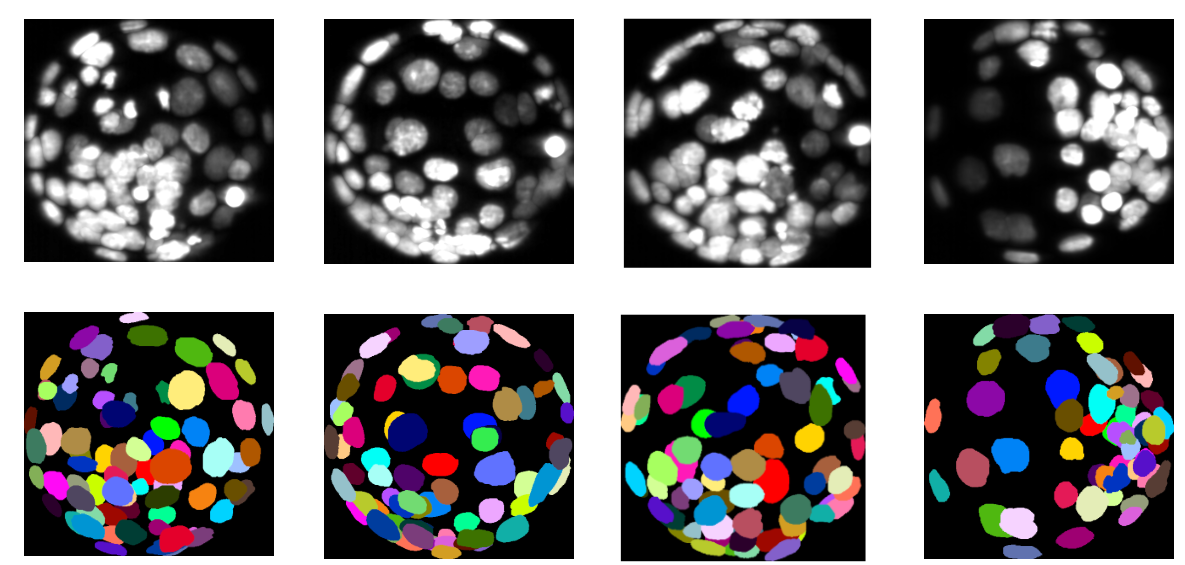
\includegraphics[width=1.0\textwidth]{Images/Methods/BlastoSPIM.png}%
    }
    \caption{Encoder embeddings of the train set clustered with k-mean and intuition of amlplified sampling \cite{LeCun.1989}.}
    \label{fig:slicing}
\end{figure}

Each image in the BlastoSPIM datasets has an xy-resolution of 0.208~µm and a z-resolution of 2.0~µm, capturing fine cellular structures across multiple focal planes. In total, 18,336 nuclei have been manually segmented, with contours drawn in every z-slice where each nucleus appears. This meticulous annotation provides precise 3D instance labels, making BlastoSPIM one of the most comprehensive resources for studying early embryogenesis and for training and evaluating segmentation models in 3D microscopy. 



\subsubsection{CTC Datasets}

The CTC dataset provides both 2D and 3D time-lapse microscopy sequences. It includes recordings of fluorescently counterstained nuclei and cells, either migrating on top of or embedded within a substrate. In addition, the dataset contains 2D brightfield, phase contrast, and differential interference contrast (DIC) microscopy videos that capture the dynamics of cells moving on flat substrates. 

Interesting, challenging datasets with very dense instances are the Fluo-N3DL datasets, which are light-sheet 3D+t images of developing insect embryo. Each image is really large and requires careful memory handling in inference. Due to the large size and density in cell instances, annotations are very limited. For every image, only a few z-slices have annotations, which usually only cover a tiny fraction of the cells present.

\begin{figure}[!ht]
    \centering
    \makebox[\textwidth]{%
    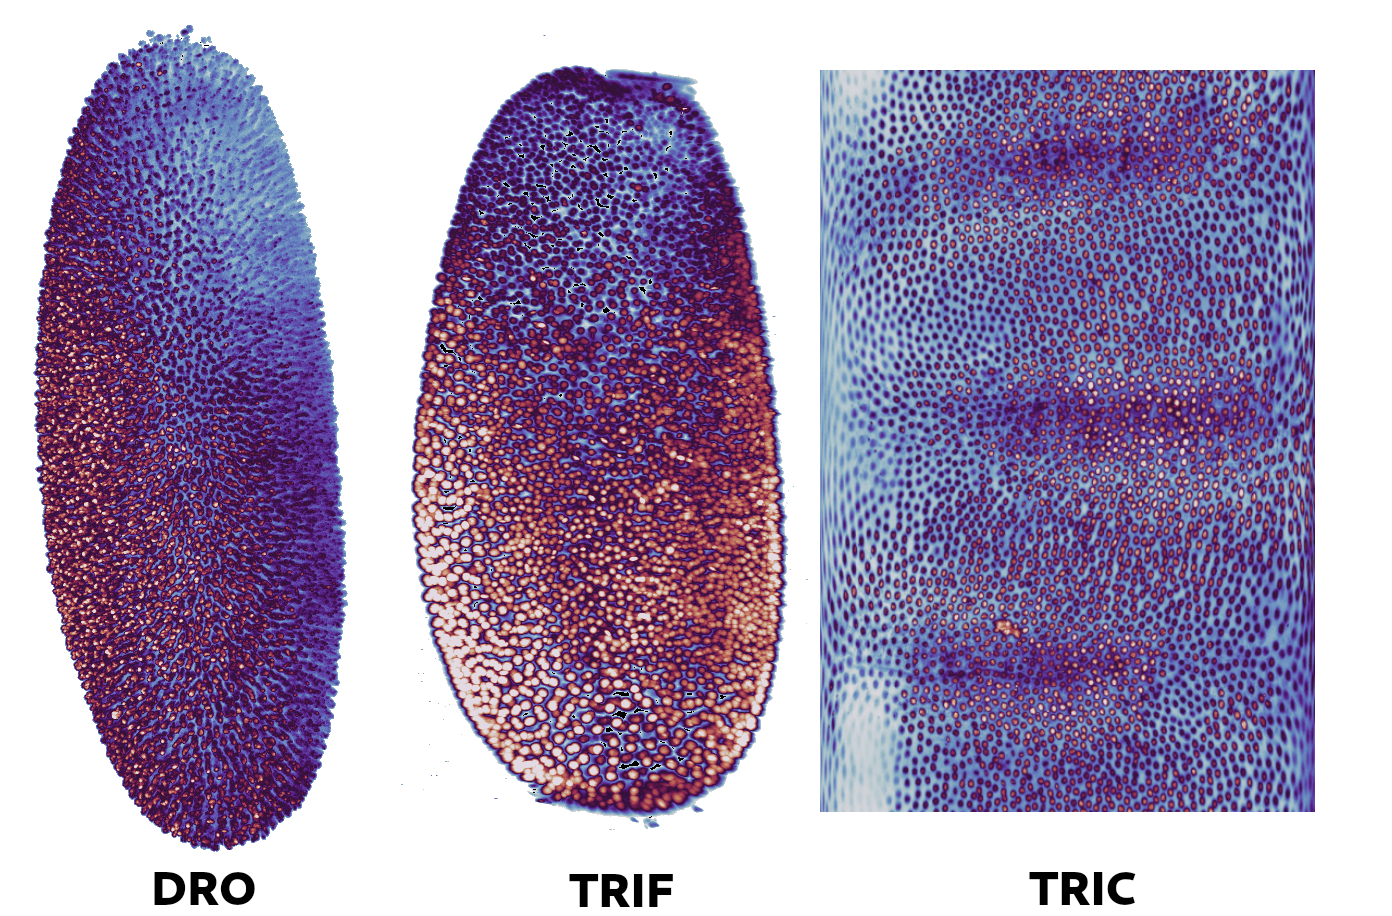
\includegraphics[width=1.0\textwidth]{Images/Methods/CTCData.png}%
    }
    \caption{Fluo-N3DL-DRO, TRIF and TRIC}
    \label{fig:slicing}
\end{figure}


We will also use some synthetic images from the Fluo-N3DH-SIM dataset, which simulates nuclei of HL60 cells stained with Hoechst. Due to the high level of noise in the data, clear boundaries are not really present, limiting the performance evaluation capabilities. 

\begin{figure}[!ht]
    \centering
    \makebox[\textwidth]{%
    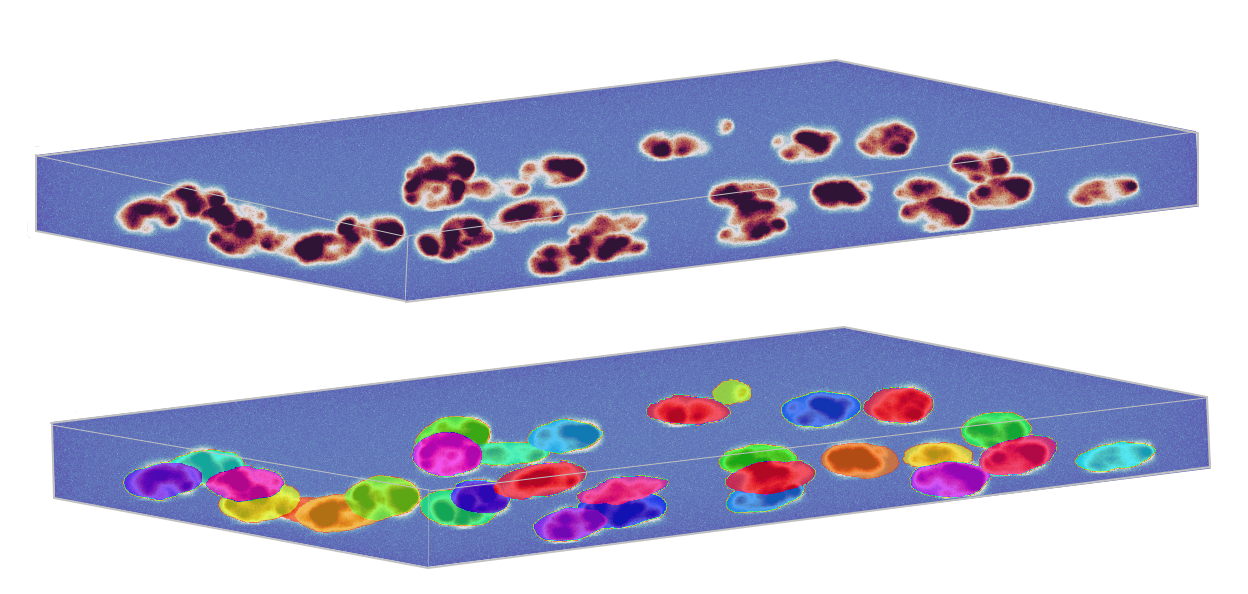
\includegraphics[width=1.0\textwidth]{Images/Methods/CTCsim.png}%
    }
    \caption{Fluo-N3DL-DRO, TRIF and TRIC}
    \label{fig:slicing}
\end{figure}





\subsubsection{Zebrafish Dataset}

This dataset captures zebrafish embryo's lateral line in 3D+t. In zebrafish embryos, the lateral line system is composed of small mechanosensory organs called \textit{neuromasts}. Neuromasts originate from cranial placodes and are deposited along the trunk and tail during early development (around 24--48 hours post fertilization). This deposition is carried out by the posterior lateral line \textit{primordium}, a migrating cluster of progenitor cells that travels from the head toward the tail and leaves behind groups of cells that mature into neuromasts. Each neuromast consists of centrally located sensory hair cells surrounded by supporting and mantle cells, which provide structural and regenerative functions. By 3--5 days post fertilization, zebrafish larvae possess a functional lateral line system with multiple neuromasts arranged in stereotyped rows. For our purposes, we focus on segmenting the migrating cluster of progenitor cells as well as the leftover neuromasts. Images are acquired with a Zeiss spinning disk and Nikon laser scanning microscope, resulting in two channels for each membrane and nuclei. Although the mebrane channel can act as a useful bias in addition to the nuclei channel in tracking, the level of noise and unclear boundaries makes the membrane channel unfeasible for segmentation. Therefore, we will primarily focus on the nuclei channel for segmentation tasks.

\begin{figure}[!ht]
    \centering
    \makebox[\textwidth]{%
    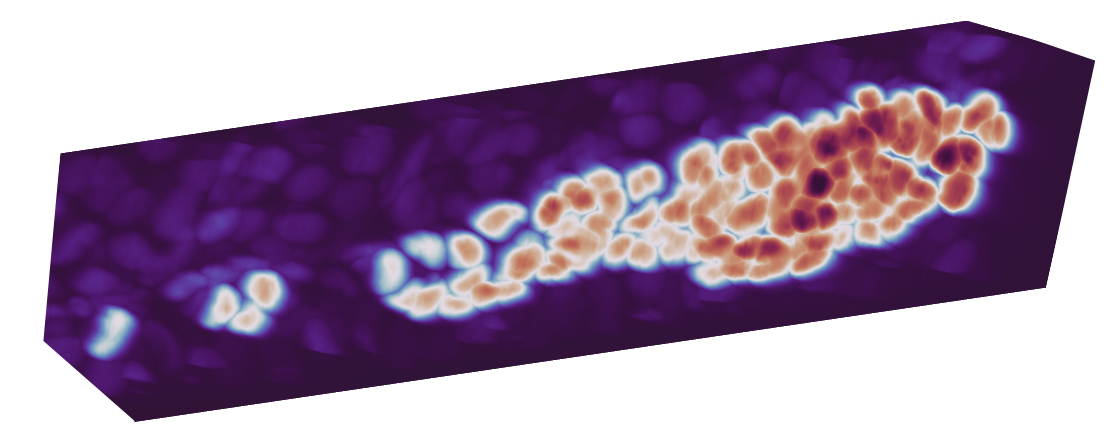
\includegraphics[width=1.0\textwidth]{Images/Methods/ZebrafishVol.png}%
    }
    \caption{Fluo-N3DL-DRO, TRIF and TRIC}
    \label{fig:ZebrafishVol}
\end{figure}

As depicted in Figure \ref{fig:ZebrafishVol}, the primordium cells can be recognized quite easily with the bare eye. This is not only due to favourable intensity contrasting, but also because of the unqiue shapes compared to the background cells. Nevertheless, if there is no bias towards the different types of cells, generalizable networks will not be able to differ forground from background cells and thus produce a lot of false positives.Although there are a lot images at different timestamps and images for wildtype variations, there is just one single 3D image labeled. Although most of our models train on 2D slice inference anyway, testing and training on the same image at different slices is rather infeasible due to strong spatial correlations between test and train data.

\begin{figure}[!ht]
    \centering
    \makebox[\textwidth]{%
    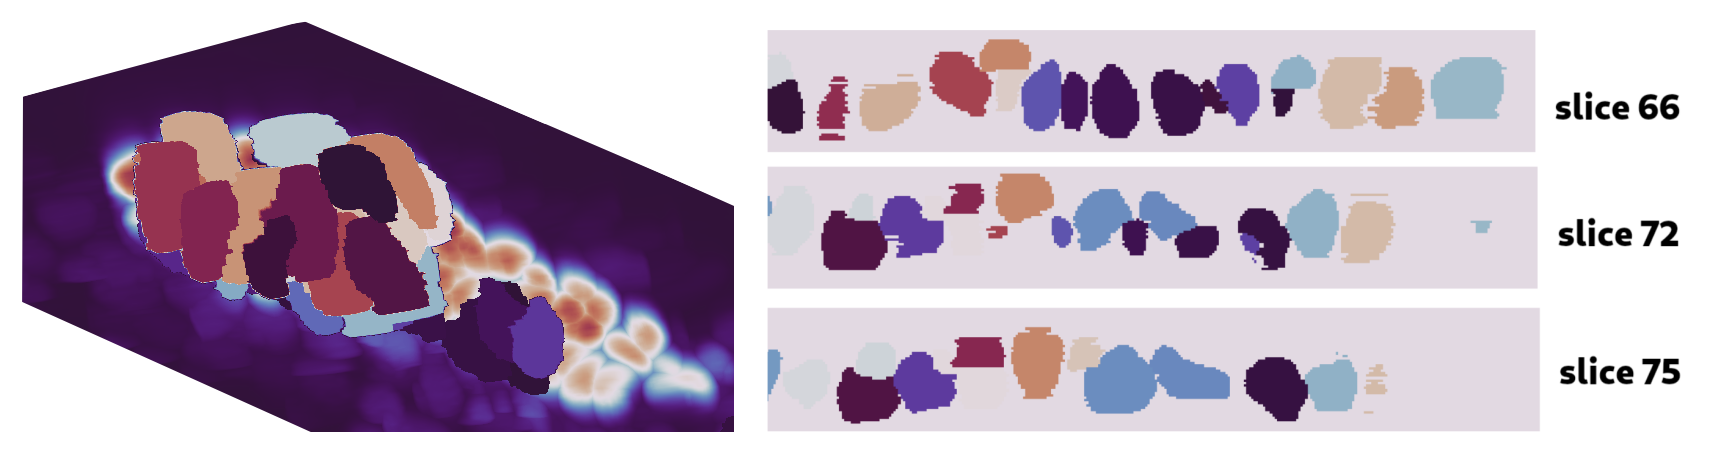
\includegraphics[width=1.0\textwidth]{Images/Methods/ZebrafishAnnotations3d.png}%
    }
    \caption{Fluo-N3DL-DRO, TRIF and TRIC}
    \label{fig:ZebrafishAnnotations3d}
\end{figure}

Another challenge with this dataset is not only that there is just one annotated image, but that the segmentation quality also impaired by the way the annotation was created. As it can be easily spotted in \ref{fig:ZebrafishAnnotations3d}, there are inconsistencies in cell annotations towards different z slices. Most likely, the annotator marked cells in just axial direction, leaving out annotations on some slices, while on some z slices further they are marked again. Also, the boundary sizes are inconsistent over z. This is particularly crucial, as our models predict slices in axial, sagital and coronal directions. So when slicing through x for example, the inconsistencies will create distortions in the flow feature space, which is aggregated from all inference directions.



\section{Mediar3D}

In this section, we introduce a way of extending Mediar to 3D. First, we present a way of using predictions along different image reslices, to compute a 3D flow field, which can be post processed into 3D predictions. We will briefly introduce challenges that go along with this method and discuss the feasibility of extending Mediar to true 3D. This would correspond to an architecture that learns actual 3D features during training.

\subsection{3D Flowfield Prediction}

For the extension to 3D flow predictions, we adapt the flow accumulation of Cellpose. For 2D inference, a two-dimensional vector field is predicted. A simple way to perform inference on 3D data, would be to loop over the depth $z$ of the image, to obtain the vertical and horizontal flows $dx$ and $dy$ related to $z$. Now when permuting the spatial dimensions to slice over $x$ instead of $z$, essentially treating $x$ as the new depth dimension, one obtains the $dy$ and $dz$ flows. Finally, repeating this over the $y$ dimension grants $dx$ and $dz$. While this sounds very intuitive, it is important to keep track of the correct way of inversely permuting the flows back to the original coordinate system. This is achieved by accumulating them into a resulting 3D flow-field vector at the correct indices. To threshold invalid flows, predicted cell probabilities are accumulated along flows as well.

\begin{algorithm}
\caption{3D Flow Accumulation with Iterative Permutations}
\label{algo:3dflows}
\begin{algorithmic}[1]
\STATE Initialize 3D flow-probability volume $\mathbf{F} \in \mathbb{R}^{4 \times H \times W \times D}$ with zeros
\STATE Define permutations $\pi_p$ and inverse permutations $\pi_p^{-1}$ for $p \in \{x,y,z\}$
\FOR{each spatial dimension $p \in \{x,y,z\}$}
    \STATE Permute input volume $I$ to $I^p = \pi_p(I)$
    \FOR{each slice $s$ along depth of $I^p$}
        \STATE Compute 2D flow $\mathbf{f}_s = (dx_s, dy_s)$ and cell probability $P_s = \sigma(I_s)$ via 2D inference
    \ENDFOR
    \STATE Stack slices to form 3D block of flows $\mathbf{F}^p \in \mathbb{R}^{4 \times H \times W \times D}$
    \STATE Inversely permute flows back: $\mathbf{F}^{p}_{\text{orig}} = \pi_p^{-1}(\mathbf{F}^p)$
    \STATE Accumulate: $\mathbf{F} \gets \mathbf{F} + \mathbf{F}^{p}_{\text{orig}}$
\ENDFOR
\RETURN $\mathbf{F}$ (final 3D flow field and cell probability map)
\end{algorithmic}
\end{algorithm}
\begin{figure}[!ht]
    \centering
    \makebox[\textwidth]{%
    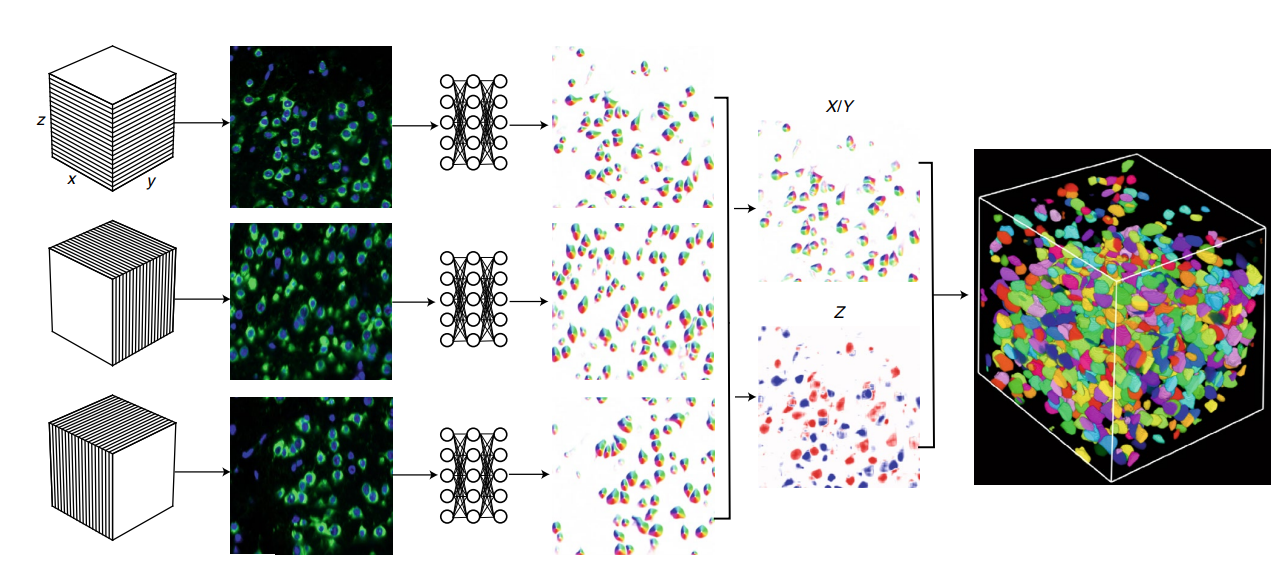
\includegraphics[width=1.0\textwidth]{Images/Methods/zflow.png}%
    }
    \caption{Encoder embeddings of the train set clustered with k-mean and intuition of amlplified sampling \cite{LeCun.1989}.}
    \label{fig:slicing}
\end{figure}

\subsection{Post-Processing of 3D Flows} %todo, removebadflowmasks

We now take a look at computing instance masks. Given the network forward outputs, we optain spatial gradients $\mathbf{dP} \in \mathbb{R}^{3 \times L_z \times L_y \times L_x}$ and cell probabilities $\mathbf{P} \in [0,1]^{L_z \times L_y \times L_x}$ to process the resulting cell instances. Candidate voxels are first identified by thresholding the probability map, defining the foreground region
\begin{equation}
\Omega = \{ (z,y,x) \mid \mathbf{P}(z,y,x) > \tau_p \},
\end{equation}
where $\tau_p$ is the cell probability threshold. For each voxel $(z,y,x) \in \Omega$, the position is iteratively advected along the predicted flow vectors according to
\begin{equation}
\mathbf{p}_{t+1} = \mathrm{clip}\!\left( \mathbf{p}_{t} + \mathbf{dP}(\mathbf{p}_{t}), \, -1, 1 \right),
\end{equation}
where $\mathbf{p}_t \in \mathbb{R}^3$ denotes the normalized voxel position at iteration $t$. The integration is performed for a fixed number of steps $T$ (typically $T=200$) using Euler dynamics, which drives voxels belonging to the same object towards common attractors in the flow field. The final positions $\mathbf{p}_T$ of all advected voxels are accumulated into a discrete histogram volume
\begin{equation}
H(\mathbf{u}) = \sum_{i=1}^{|\Omega|} \delta(\mathbf{p}_T^{(i)} - \mathbf{u}),
\end{equation}
where $\delta(\mathbf{p}_T^{(i)} - \mathbf{u})$ acts as a one-hot indicator function that evaluates to $1$ if the advected voxel $\mathbf{p}_T^{(i)}$ coincides with the discrete location $\mathbf{u}$ and to $0$ otherwise. Local maxima of $H$ are detected by $n$-dimensional max pooling with kernel size $5$, and peaks with histogram counts above a fixed threshold are retained as seeds, which represent candidate cell centers. Around each seed, a local neighborhood of size $11 \times 11 \times 11$ voxels is extracted and iteratively expanded using morphological max pooling under the constraint $H(\mathbf{u}) > 2$, thereby forming seed masks corresponding to attraction basins of the detected maxima. The converged voxel positions $\mathbf{p}_T$ are then mapped to these seed regions, and each voxel in $\Omega$ is assigned a label $m \in \{1,2,\dots,N\}$, where $N$ is \#detected seeds. This produces an initial labeled segmentation.
Finally, masks that are larger than a fraction $\tau_s$ of the total image volume are discarded, very small masks are removed and filled, and masks that exhibit insufficient alignment with the flow vectors are pruned using a flow-consistency criterion. Remaining masks are renumbered to enforce consecutive integer labels, resulting in the final instance segmentation.


\section{Segmentation Network Design Choices}

In this section, we introduce different approaches to improve the Mediar architecture by using different encoder and decoder building blocks. First, we will sketch the fundamental structure of our segmentation networks on a high-level view. Based on this concept, we will be build new models by modifying indivial components. Inspired by the release of CellposeSAM, we will present a model that uses the SAM2 pretrained Hiera image encoder instead of the SegFormer MiT blocks for the Mediar Network. Furthermore, we will consider the use of plain convolutional decoder blocks instead of the MA-Net decoder. We will also attempt to reason the rationale behind these design choices and, in doing so, set our expectations for the resulting performance of the network modifications.

\subsection{High-Level Network Design}

In this subsection, we deduce some general concepts to our network design and point out their design choices on a high level. As previous work such as CellposeSAM, Mediar and other segmentation networks suggest the encoder-decoder style learning, we adapt this as our underlying concept for our network architecture. 

For the encoder part, the image is transformed into a latent feature space by alternating channel size while downsampling spatial dimensions as the network gets deeper. From a high-level perspective, this can be regarded as a module $E(\mathbf{I})$, that inputs an image $\mathbf{I} \in \mathbb{R}^{3 \times H \times W}$ and outputs a tuple of multiple feature spaces:

\begin{equation}
E(\mathbf{I}) =
{\mathbf{F}_i \in \mathbb{R}^{C_i \times H/{2^i} \times W/{2^i}} \mid i = 1, \dots, N },
\end{equation}

where the tuple $\mathbf{F}_i$ may contain an arbitrary number of feature resolutions $i$, each with its own channel dimension $C_i$ and spatial size $H \times W$. Note that while it is not necessary to reduce spatial size to integer powers of 2, this is commonly the case due to the nature of downsampling mechanisms such as strided convolutions or pooling operations.

The decoder fuses all information gathered by the encoder into an overall network prediction by mapping the features to the learning objective of the network. This includes upsampling the spatial dimensions back to pixel space and reducing the channel dimensions to the desired output shape. From a high-level perspective, the decoder can be written as a mapping

\begin{equation}
D({\mathbf{F}_i}) = \hat{\mathbf{Y}} \in \mathbb{R}^{C\text{out} \times H \times W},
\end{equation}

where $C_\text{out}$ denotes the number of output channels, depending on the learning objective. In semantic segmentation, this corresponds to the number of semantic classes, with a softmax distribution assigning each pixel to a class. For cellular instance segmentation, the decoder instead maps the features to outputs such as flow fields or probability maps, which are subsequently post-processed into instance masks, as done in StarDist or Cellpose.

Beyond this high-level network layout, which already involves many design decisions, each building block obviously contains numerous other parameters and layer configurations that must be carefully chosen. But focussing on the above mentioned high-level design criterions is important to keep track of the bigger picture when it comes to a large change in network layout, which will be presented in the following subsections. Understanding the changes made on the above described high-level layout, will make a seemingly completely new architecture, very tangible and the low-level design choices a lot more intuitive.

For instance, the authors of Cellpose launched a completely revised version of their network a few weeks after the start of my thesis. What seems to be a major rework of their repository, turns out to be just a few lines of code, as they barely touch the low-level components of the modules they take from established methods. So from a high-level view, they switched the CNN based encoder part of their network with the image encoder of SAM1, and used just a single 1x1 convolutional layer (along non-learnable layer to convert patch- to pixel space) to fuse their single resolutional feature map to the cellpose learning objective.



\subsection{SAM2 Encoder Registry}

First, we want to setup experiments using the Hiera encoder of the SAM2 model instead of the SegFormer encoder blocks for the Mediar model. The SegFormer backbone blocks are composed of multiple Mix Transformer(MiT) blocks with consecutive overlapping patch merging, efficient self-attention and Mix-FFN, which provide multi-scale features due to the patch merging process at multiple stages. From a high-level perspective, the MiT B5 encoder blocks produce 4 feature maps with different channel sizes and spatial resolutions. 
The Hiera image encoder is composed of standard ViT blocks, except global attention is replaced by Mask Unit Attention at shallow layers with high spatial resolution. A total of 3 pooling layers enables the encoder to output features at four different resolutions. This excatly matches the SegFormer encoder outputs on a high-level, except the feature maps produced by the Hiera encoder all have 256 channels, whereas the feature maps of the MiT B5 module all have increasing channel sizes for deeper feature maps. Note that also the default config used to build the SAM2 registry defines a parameter that makes the image encoder discard the lowest resolution feature after forwarding the neck, resulting in only 3 feature resolutions instead of 4. Hardcoding this value or editing the default registry config fixes this problem because the powerful pretrained weights from the SAM2 registry are not effected by the amount of feature outputs of the image encoder. This is because the features are computed in the forward pass regardless of the parameter that discards them afterwards by parameterized indexing in the neck forward function.

\subsection{Merging SAM2 Image Encoder with Mediar}

The actual integration of the SAM2 model into the Mediar network architecture is not too difficult if conducted carefully with debugging tools. Challenging aspects include dealing with cryptic, undocumented backend code of MA-Net and MixTransformer and more importantly, editing the MA-Net blocks with regard to numerical stability and compability with the SAM2 registry. Pseudo QKV operations in the PAB Block of the MA-Net decoder are now normed with respect to the embedding dimension as suggested in \ref{attentionisallyouneed}, to prevent float16 overflow in network training. Also, MA-Net assumes the first feature to be the encoder input image and thus discards the shallowest feature per default. This is now adjusted to match the backbone outputs from Hiera. Skip connections have been removed for the Decoder Block 1, as this block was connected to a dummy feature from the SegFormer output. 

\subsection{Lightweight Decoder}

Many segmentation networks \cite{Segformer, CellposeSAM} have shown great performance without relying on heavy-weight decoder modules such as it is the case for Mediar and its MA-Net decoder blocks. We therefore want to conduct experiments using leight-weight decoder blocks and the SAM2 image encoder. 

The decoder blocks take a feature map as input and a skip connection from the encoder if there it is not the center block. The input is first upsampled by a factor of two using nearest-neighbor interpolation. When a skip connection is provided, the upsampled features are concatenated with the skip features along the channel dimension, increasing the input dimensionality of the subsequent convolution. The combined tensor is then processed by two sequential conv2dReLU units, each consisting of a $3 \times 3$ convolution with padding of $1$, followed by a ReLU activation, and a batch normalization layer. The first convolution reduces the concatenated feature channels to the target output dimensionality, and the second further refines the representation while maintaining the same number of channels. This design focusses on spatial resolution recovery and integration of encoder features at corresponding scales, without using the heavy-weight pseudo attention modules of the MA-Net. 




\section{Training Challenges and Solutions}

In this section we will analyse the training procedure of our networks. First, the general training pipeline is outlined, describing the main components. After setting the baseline for cellpose learning objective training, we will look into challenges that come along training with only partly annotated data. 

\subsection{Training Pipeline}

Now we look into the general pipeline for our network training. In general, we want to train our models in such a way, that it is capable of performing well on zero-shot predictions. To achieve this, we follow the approach of previous work about generalizable model training. This includes \textit{pretraining} the data on a large, diverse dataset. This model can be further \textit{finetuned} on a specific downstream modality. The original Mediar training config suggests a multi-phase training of two seperate models that predict in an ensembling manner (this multi-phase training is described in \ref{chapter:Mediar}). Since this multi-phase training is tailored for the best performance on a large challenge dataset, this method is unsuitable for small target datasets, especially if the target datasets have limited annotations. Within this thesis, we therefore aim to produce a single phase, generalizable model, which Mediar refers to as their \textit{from\_phase1.pth} model.

\subsubsection{Data preperation and sampling}
Since pretraining and finetuning share mostly the same pipeline, adjustments should be configured in a seperate train config json file. The main difference between pretraining and finetuning configs lies the data preperation and sampling. Pretraining mainly focusses on using a very large, diverse dataset. This can also be improved, by the discovery of latent modalites, as the original Mediar paper suggests \ref{fig:latent_modalities}. By clustering the encoder embeddings from the phase-1 pretrained model using k-means with 40 clusters, they amplify the sampling ratio in favour of underrepresented modalities. We adapt this method as the majority of pretraining images are worm images from the Livecell-dataset. Other than the amount of data, it is also important to handle the dimensionality of the target data for the finetuning. Since we want to finetune our model to perfrom well on specific 3D data, we train our model to predict the 2D flows and cell probablities on the 2D slices of the volume in each orientation. This requires to prepare slices of the 3D finetuning data for every direction. 


Loading the training data into the training pipeline requires the mapping of train images and ground truth masks to json file. This is done via a modified version of the mediar mapping script, which enables the user to map multiple datasets at once, without naming constraints. The json files are loaded and split into train and validation data with a custom dataloader, that is configured via user inputs defined in a seperate train config json file. Using the monai package, which is a precompiled library for biomedical image processing, certain train and validation transformations are defined in the dataloader to augment the batch data once its loaded in a training iteration.

\subsubsection{Forward pass}
After loading the batch data in each training epoch, the network forward pass predicts 2D flows and cell probability logits, which are passed into the metric function to compute the loss. For the ground truth data, the flow representation is computed runtime. While this sounds very inefficient, precomputing the flow ground truths comes along with a few challenges. The precomputed flows have to be integrated into the dataloading pipeline. This includes applying the same spatially deforming augmentation transformations to the flows as the training data. Since the flow generation of ground truth data is not invariant to all spatial transformations, the precomputed flows dont match the flows computed at runtime after the transformation. The unit test for this matter has shown, that in most cases the reconstructed masks from the precomputed and runtime computed flows differed significantly, while the time costs saved was in the magnitude of a few milliseconds per epoch, partly because the dataloading and augmentation of the precomputed flow has to be substracted from the time it takes to generate the flows runtime. Although these few milliseconds scale up pretty quickly to a 1-2 hours for 80 epochs at 5500 iterations per epoch, the performance loss can not be justified. Eschweiler et al \cite{eschweiler} suggested to simplify the learning objective to a variant of the tanh to speed up the expensive generation of flows at neglectable performance loss. While this might be a promising alternative, it has not been implemented and tested yet.

With runtime computed ground truth flows, the loss can be calculated after the forward pass with a binary cross-entropy term for the cell probabilities and a mean squared error term for the flow components:

\begin{equation} 
\mathcal{L} \;=\; \| \hat{y}_0 - 5 F_x \|^2 \;+\; \| \hat{y}_1 - 5 F_y \|^2 
\;+\; \mathcal{L}_{\text{BCE}} \bigl(\sigma(\hat{y}_2), P \bigr),
\end{equation}

Here, $\hat{y}_0$ and $\hat{y}_1$ denote the predicted horizontal and vertical flow channels, while $F_x$ and $F_y$ represent the corresponding ground-truth flow fields. The term $\hat{y}_2$ refers to the raw (logit) prediction of the cell probability map, and $P$ denotes the ground-truth binary mask of cell locations. The function $\sigma(\cdot)$ corresponds to the sigmoid activation, which maps logits to probabilities, and $\mathcal{L}_{\text{BCE}}(\cdot,\cdot)$ is the binary cross-entropy loss between the predicted and ground-truth probabilities. The ground-truth flows are scaled by a factor of $5$ to match relative contribution of the L2 loss and cross-entropy loss. Although it may seem like a semantical error to scale the ground truth flows before substraction, it works well in practice. Unfortunetely, there was no explaination given in the paper on why they implemented it like this. A raised github issue addressing this issue remained unanswered. Usually, it is common to scale loss contributions after the whole loss component is calculated. Either way, experiments with a different way of scaling the loss contribution have shown no difference in performance.  


\subsubsection{Backward pass}


In practice, we implemented the individual loss components are computed seperately for logging purpose, which can be handy to tune the weighting of the loss components. Interestingly, the Mediar code logs the summed loss components as dice loss, although the dice loss is neither computed in valid epochs, nor in the training iterations. We log the loss to Weights and Biases, which is an interactive cli and webtool that can be integrated into the training pipeline to plot losses and performance while training. It can be used for free with an academic license. The per-pixel MSE flow and BCE cell probablity loss is aggregated into a scalar value with the build-in mean reduction method from torch and backpropagated with the AdamW optimizer.

\vspace{1em} % or 2em, adjust as needed

Since all networks share the same learning objective, the training pipeline can be mostly reused. Apart from hyperparameters that depend on the network's feature aquisition and amount of pretraining, the metric function and dataloading including the module for ground truth flow generation stays the same. So the pipeline is used for all networks, but  changes in the way the loss is computed, depending on is the training data is fully annotated. How these challenges are faced, will be described on the following subsection.

\subsection{Training with Limited Annotations}

Since 3D data labeling is an expensive task, many challenge or use-case datasets are only labeled partially, as described in \ref{chapter:3.1}. Since oftentimes this is the only resource to significantly improve the zero-shot performance for these target datasets, we will look into ways to finetune our networks with limited annotations. 

\subsubsection{Using Unsupervised Learning Methods}

Previous work has explored various strategies to incorporate large sets of unlabeled images into training. For example, the Mediar framework investigated several semi-supervised approaches, including consistency regularization with strong data augmentations, reconstruction losses with an auxiliary head (both restricted to the cell regions and over the full image), and pseudo-labeling from pretrained or fine-tuned models. However, these attempts did not yield improvements over training with labeled data alone, leading the authors to ultimately rely only on the annotated subset. This highlights the difficulty of leveraging unlabeled data effectively in training and motivates alternative approaches.

\subsubsection{Masked Loss Function}

Finetuning the models with limited annotations, requires careful evaluation of network forward passes. Naively applying BCE and MSE loss to the predictions will punish false positives a lot, in case only a few instances are labeled. Not only will the contour accuracy decrease, but the arbitrarely labeled instances will make it impossible for the network to make distinctions for true and false positives as epochs progress. To decrease gradient distortions of unlabeled areas, the image shown to the network in forward pass can be cropped to a ROI, corresponding to a bounding box of a few nearby instance labels, with some spare buffer spaces to provide some image context. While this heavily reduces the effects of the majority of the unlabeled image parts, this approach is still prone to gradient distortions in cases of dense cell regions, where a buffered bounding box can not be established without including unlabeled instances.

To prevent false network weight gradient flow due to pseudo false positives completely, one could crop the image to individual cell instances without buffer space to prevent gradient distortions by unlabeled neighboring cells. While this is not always feasible, especially in really dense cell distributions, this also prevents the network to learn spatial context features of the cell instances. As the instance cropped images has to be padded severely to fit the input dimensions of the network, the network would mostly see zero values around the cell. This could lead to even worse feature learning, especially because the receptive field of transformer based encoders can be global.

Another way of dealing with the gradient contribution of unlabeled regions would be to define a supervision mask, that sets the loss to zero for regions, where no annotations are present. As there would be no false positive feedback loss contribution for the case that the loss is only calculated for positive regions, it is necessary to somehow extend the region of loss contribution beyond labeled regions. In order to not only get false negative feedback, the supervision mask for the loss could be extended with binary operations such as dilation. The kernel size for dilation and the amount of iterations for consecutive dilation, have to be carefully tuned, as potential pseudo false positive can be introduced again. This can be handled again by introducing some sort of distance weighting of the loss mask around the labeled region. The loss contribution could for example decay linearly by the cartesian distance, or even in a guassian manner. Note that the tuning of the parameters such as dilation iterations, kernel size and distance weighting are heavily depended on the specific dataset.




\section{3D Feature Network}

In this section, we investigate a few strategies to encourage the network to learn 3D features. First, we look into a method of adding 3D flow gradients to the loss. Then, we shortly discuss the feasibility using 3D building blocks for the encoder and decoder. Lastly, we build a new architecture that encodes 2D slice features and uses them to learn 3D features in the decoder path, using 3D convolutions. 

\subsection{3D Gradient Flow Training}

We first look into a method of adapting the same 3D flow aggregation technique for training, as it used for inference. The idea of 3D flows is, to slice a volume into 2D slices for every cartesian direction $(x, y, z)$, forwarding them into the network to predict 2D flows for every direction, to then be able to aggregate them into 3D flows. This can be integrated into finetuning, given that 3D instance annotations are provided. The 3D flow loss requires multiple consecutive slices to be forwarded within one batch, to then calculate 3D flows and getting three MSE flow loss components. The algorithm is summerized in Algorithm~\ref{algo:3Dflowtraining}. In case of unlabeled regions, the same loss masking could be applied as described in the previous section.

\begin{algorithm}[H]
\caption{Training with masked 3D flow loss}
\label{algo:3Dflowtraining}
\begin{algorithmic}[1]
\FOR{each optimizer step}
    \STATE Load one 3D image $I$ and its mask $M$
    \STATE Slice $I$ into 2D images along YX, ZY, and ZX directions to form a batch $B$
    \STATE Perform a forward pass of $B$ through the network to obtain predictions $\hat{B}$
    \STATE Using knowledge of YX, ZY, and ZX indices in $\hat{B}$, compute 3D flows $\hat{F}$
    \STATE Compute masked MSE loss between $\hat{F}$ and ground-truth flows $F$
    \STATE Update network parameters via backpropagation
\ENDFOR
\end{algorithmic}
\end{algorithm}

While this approach sounds quite logical at first, there are a few issues. First and most importantly, as the network still forwards 2D slices, there are no actual 3D features learned like it would be the case for the 3D Cellpose network proposed by Eschweiler et al. In our setup, the incorporation of 3D flows in the loss metric function primarily acts as a regularizer. While it does encourage consistency of predicted flows across slices in all three spatial directions, it doesnt make use of the 3D annotations to learn actual 3D spatial features. Another drawback of this method is, that loading even subvolumes in a sliding window manner quickly becomes very memory expensive. In practice, comsumer grade GPUs can not handle more than a batch size of 9 with all network weights at the same time for training. Due to these limitations, we decided to not persue this approach any longer.  

\subsection{Feasibility of Extending Mediar to True 3D}

Since the proposed network of Eschweiler et al. has shown great performance in learning true 3D features, by using 3D convolutional layers, it seems reasonable to extend the encoder and decoder components of Mediar to true 3D. While this would not be technically impossible, as previous work has successfully implemented 3D attention layers for image segmentation \cite{Primus}, global attention in 3D would severely influence computational complexity. More importantly, training these blocks from scratch would require a lot of annotated 3D training data, due to the lack of inductive bias in the architecture. We would ultimately lose the strong generalizable power from the heavily pretrained 2D encoders. Since pretraining data for 3D cellsegmentation is in the magnitudes of a few hundrets, this approach seems unlikely to succeed. As Carsen Stringer, the original author of cellpose suggests, CNNs would definetely be more suitable for training a true 3D cellpose variant from scratch because of the above mentioned reasons.

\subsection{Hybrid Approach for Learning True 3D Features}

In this subsection, we present a different approach for learning true 3D features. We adapt the design of xy et al \cite{3dfeautreslicingpaper}, who keep the strong pretaining power of a foundational encoder and train a seperate 3D convolutional decoder to learn 3D features based on the forwarded slices of the 2D encoder.

Specifically, they used the SAM1 image encoder registry as the encoder and a lightweight decoder. The input image
\(
I \in \mathbb{R}^{H \times W \times D}
\) 
is sliced along the depth dimension, converted to a 3-channel image and forwarded through the encoder. The resulting slice embeddings $F = [f_1, f_2, \dots, f_D] \in \mathbb{R}^{\frac{H}{16} \times \frac{W}{16} \times D \times 256}$ are stacked to form a 3D feature volume \(F\), which is then processed by the 3D decoder to capture depth-wise relationships and map the features to the Cellpose learning objective. The forward pass is summarized in Algorithm~\ref{algo:sam3d_forward}.

\begin{algorithm}[H]
\caption{Hybrid 3D Feature Network Forward Pass}
\label{algo:sam3d_forward}
\begin{algorithmic}[1]
\REQUIRE Volumetric input $I \in \mathbb{R}^{H \times W \times D}$
\ENSURE Cellpose learning objectives $\hat{Y} \in \mathbb{R}^{H \times W \times D}$

\STATE Split $I$ into $D$ slices along the depth axis: $I = \{I_i\}_{i=1}^{D}$, $I_i \in \mathbb{R}^{3 \times H \times W}$
\FOR{$i = 1$ to $D$}
    \STATE Compute slice embeddings: $f_i = \text{Enc}(I_i)$ \COMMENT{$f_i \in \mathbb{R}^{H/16 \times W/16 \times 256}$}
\ENDFOR
\STATE Stack slice embeddings to form 3D feature volume: 

$F = [f_1, f_2, \dots, f_D] \in \mathbb{R}^{H/16 \times W/16 \times D \times 256}$
\STATE Pass the stack embeddings to the 3D decoder layers: 
\FOR{$block$ in $DecoderBlocks$}
\STATE  
$\hat{Y} = \text{block}(F)$
\ENDFOR
\RETURN $\hat{Y}$
\end{algorithmic}
\end{algorithm}
To further tailor this method for our purpose, we take not only the pretrained SAM1 image encoder registry, but also use the weights from the pretrained CellposeSAM encoder, that should already be quite potent for providing cell segmentation slice embeddings. We therefore dont need to train the encoder seperately and freeze the weights completely, while training the 3D decoder from scratch. 

Although this approach performed well on medical image segmentation, there are still some potential drawbacks of this hybrid method. As the 3D decoder is trained from scratch, a lot of 3D annotated data will be needed which is not always available for specific datasets. Also, strong performance across multiple modalities, particularly on modalities not present during training, is not expected for the amount of pretraining data available. Potential cures for that matter could be diffusion models that synthesize large amounts of fully annotated training data. This has not yet been tested.